\documentclass[border=3pt]{standalone}
\usepackage[utf8]{inputenc}
\usepackage[T1]{fontenc}
\usepackage{lmodern}
\renewcommand{\familydefault}{\sfdefault}
\usepackage{sansmath}\sansmath
\usepackage{chemfig}
\usepackage{pgfplots}\pgfplotsset{compat=1.18,/pgf/number format/use comma,/pgf/number format/1000 sep={.}}
\usetikzlibrary{arrows.meta,calc,positioning,decorations.pathmorphing,patterns}
% paleta del sitio
\definecolor{nar}{HTML}{E8680C}\definecolor{narc}{HTML}{FFB35C}\definecolor{hielo}{HTML}{FFF3E8}
\definecolor{tinta}{HTML}{1D1D1F}\definecolor{gris}{HTML}{6E6E73}\definecolor{lila}{HTML}{7C5CF0}
\definecolor{azul}{HTML}{2F6FD6}\definecolor{menta}{HTML}{17A673}\definecolor{coral}{HTML}{E8342A}
\setchemfig{atom sep=2em,bond style={line width=0.8pt}}
\tikzset{lab/.style={font=\small\bfseries,text=nar},pie/.style={font=\footnotesize,text=tinta,align=center}}
\begin{document}
\scalebox{0.9}{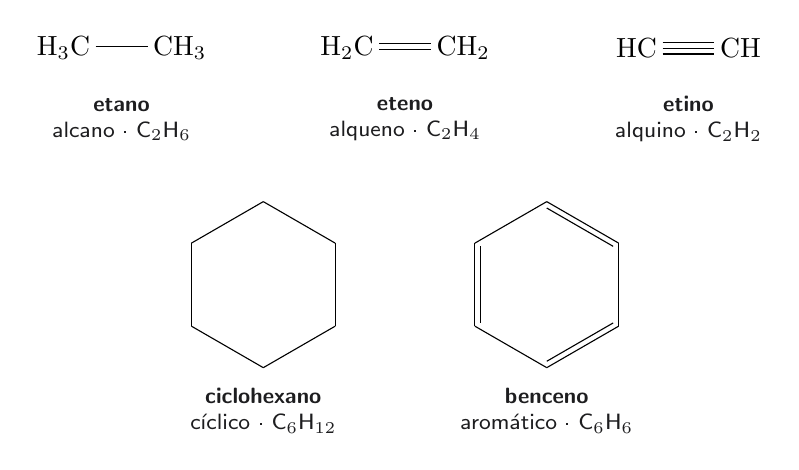
\begin{tikzpicture}
\node at (0,0) {\chemfig{H_3C-CH_3}}; \node[pie] at (0,-0.9) {\textbf{etano}\\alcano · C$_2$H$_6$};
\node at (3.6,0) {\chemfig{H_2C=CH_2}}; \node[pie] at (3.6,-0.9) {\textbf{eteno}\\alqueno · C$_2$H$_4$};
\node at (7.2,0) {\chemfig{HC~CH}}; \node[pie] at (7.2,-0.9) {\textbf{etino}\\alquino · C$_2$H$_2$};
\node at (1.8,-3.0) {\chemfig{*6(------)}}; \node[pie] at (1.8,-4.6) {\textbf{ciclohexano}\\cíclico · C$_6$H$_{12}$};
\node at (5.4,-3.0) {\chemfig{*6(-=-=-=)}}; \node[pie] at (5.4,-4.6) {\textbf{benceno}\\aromático · C$_6$H$_6$};
\end{tikzpicture}}
\end{document}
